\section{Results}
\label{sec:results}


%\begin{figure}[t]
%
%\mbox{\epsfig{figure=filename.eps,width=\linewidth,clip=}}
%
%\caption{Description of figure -- explain all elements, but do not
%draw conclusions here.}
%\label{fig:figure_label}
%\end{figure}

Let's start with the solution to equation (her trengs ref). Our general matrix solver gave the results shown in figure \ref{fig:compare} for n=10, n=100 and n=1000. The analytic solution is also shown. For n=1000 the numerical and analytical solutions are so similar that we can not distinguish them in the plot, even after zooming in with a factor of 100. 
\begin{figure}[htbp]
	\centering
	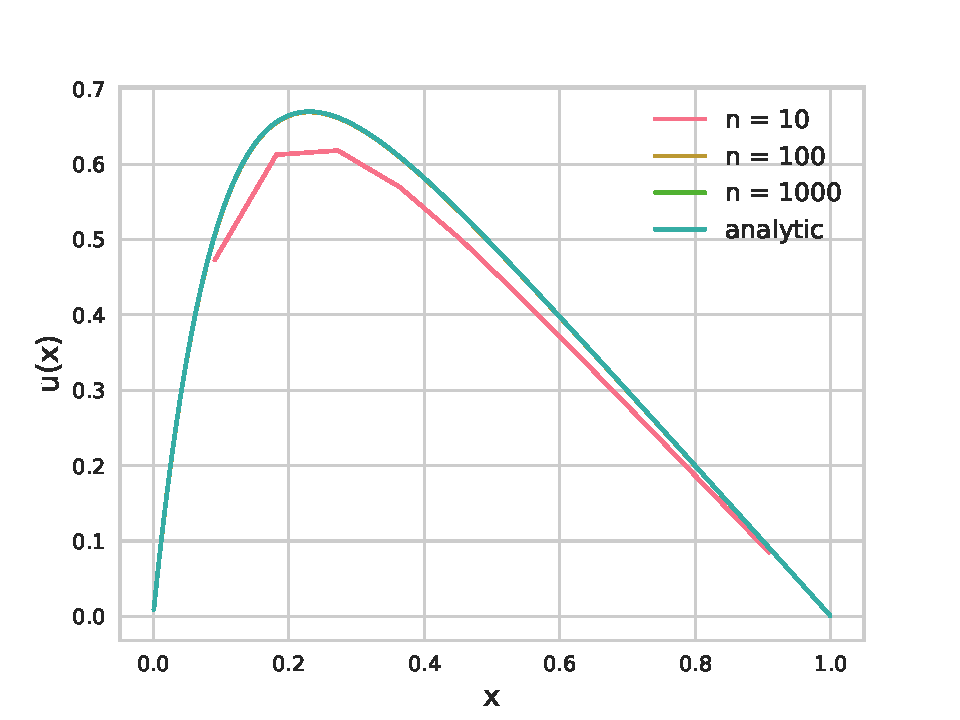
\includegraphics[width=0.5\textwidth]{general_matrix_compare.pdf}
	\caption{The numeric solution using different numbers of steps with the analytic solution. The window shows a section of the plot zoomed in with a factor of 100.}
	\label{fig:compare}
\end{figure}

Table \ref{table:time} shows the ratio between the CPU time for the general algorithm and the special algorithm, and the ratio between the LU decomposition algorithm and the special algorithm.  

\begin{figure}[htbp]
	\centering
	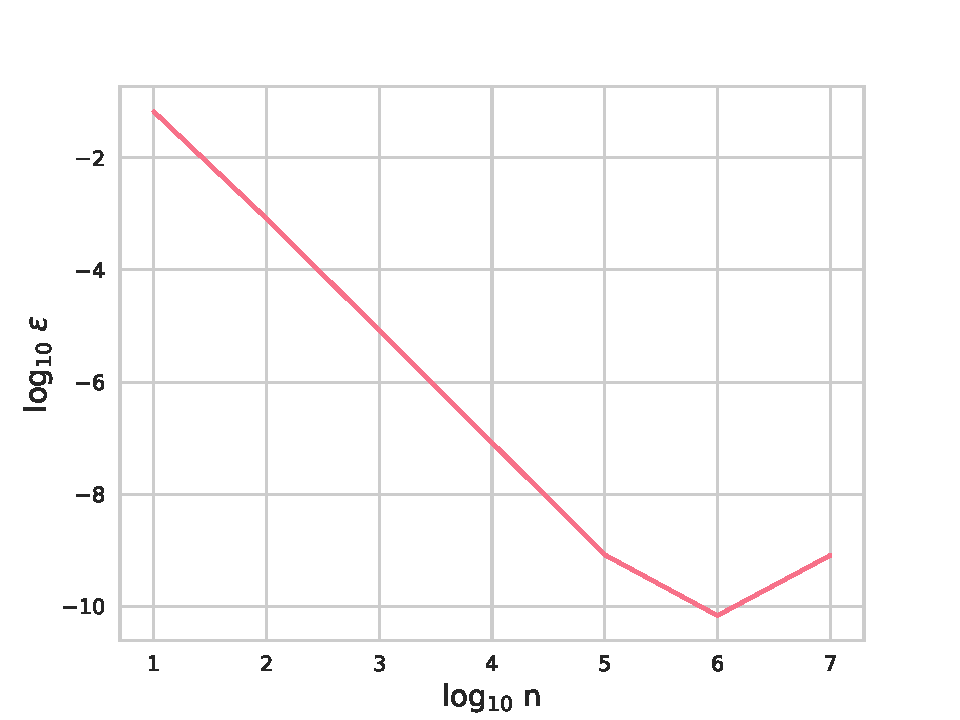
\includegraphics[width=0.5\textwidth]{error.pdf}
	\caption{The maximum error in our specialized matrix solver as a function of the number of steps/matrix size in a logarithmic scale.}
	\label{fig:error}
\end{figure}

\begin{table}[htbp]
	\centering
	\begin{tabular}{lrr}
		\textbf{n} & $\mathbf{{t_g}/{t_s}}$ & $\mathbf{{t_{LU}}/{t_s}}$  \\
		\midrule
		\addlinespace[0.1cm]
		
		10         & 2.08                                                                                          & 3.70                                                                                        \\
		$10^2$       & 1.89                                                                                          & $1.00\cdot 10^2 $                                                                                         \\
		$10^3$       & 1.48                                                                                          & $1.05 \cdot 10^4 $                                                                                        \\
		$10^4$       & 1.43                                                                                          & $1.18 \cdot 10^6$                                                                                         \\
		$10^5$       & 1.39                                                                                          & -                                                                                         \\
		$10^6$       & 1.41                                                                                          & -                                                                                        \\
		$10^7$       & 1.39                                                                                          &    -                                                                                    
	\end{tabular}  \caption{Ratio between CPU time for the general algorithm ($\mathbf{t_g}$), the special algorithm ($\mathbf{t_g}$) and the LU decomposition algorithm ($\mathbf{t_{LU}}$) for different matrix sizes (\textbf{n}). The LU decomposition crashed for \textbf{n} greater than $10^4$.} \label{table:time}
\end{table} 